\documentclass{beamer}
\usepackage[utf8]{inputenc}
\usepackage{graphicx, epsfig}
\usepackage{amsmath,mathrsfs,amsfonts,amssymb}
\usepackage{floatflt}
\usepackage{epic,ecltree}
\usepackage{mathtext}
\usepackage{fancybox}
\usepackage{fancyhdr}
\usepackage{multirow}
\usepackage{enumerate}
\usepackage{epstopdf}
\usepackage{multicol}
\usepackage{algorithm}
\usepackage[noend]{algorithmic}
\usepackage{tikz}
\usepackage{blindtext}
\usetheme{default}%{Singapore}%{Warsaw}%{Warsaw}%{Darmstadt}
\usecolortheme{default}

\setbeamerfont{title}{size=\Huge}
\setbeamertemplate{footline}[page number]{}

\setbeamertemplate{section in toc}[sections numbered]


\makeatletter
\newcommand\HUGE{\@setfontsize\Huge{35}{40}}
\makeatother    

\setbeamerfont{title}{size=\HUGE}
\beamertemplatenavigationsymbolsempty

% latin bold lower
\newcommand{\ba}{\mathbf{a}} 
\newcommand{\bc}{\mathbf{c}} 
\newcommand{\be}{\mathbf{e}} 
\newcommand{\bh}{\mathbf{h}} 
\newcommand{\bp}{\mathbf{p}} 
\newcommand{\bt}{\mathbf{t}} 
\newcommand{\bs}{\mathbf{s}} 
\newcommand{\bu}{\mathbf{u}} 
\newcommand{\bv}{\mathbf{v}} 
\newcommand{\bw}{\mathbf{w}} 
\newcommand{\bx}{\mathbf{x}} 
\newcommand{\by}{\mathbf{y}} 
\newcommand{\bz}{\mathbf{z}} 

% latin bold upper
\newcommand{\bA}{\mathbf{A}} 
\newcommand{\bB}{\mathbf{B}} 
\newcommand{\bC}{\mathbf{C}} 
\newcommand{\bI}{\mathbf{I}} 
\newcommand{\bJ}{\mathbf{J}} 
\newcommand{\bL}{\mathbf{L}} 
\newcommand{\bM}{\mathbf{M}} 
\newcommand{\bQ}{\mathbf{Q}} 
\newcommand{\bT}{\mathbf{T}} 
\newcommand{\bU}{\mathbf{U}} 
\newcommand{\bV}{\mathbf{V}} 
\newcommand{\bW}{\mathbf{W}} 
\newcommand{\bX}{\mathbf{X}} 
\newcommand{\bY}{\mathbf{Y}} 
\newcommand{\bZ}{\mathbf{Z}} 

% latin cal upper
\newcommand{\cG}{\mathcal{G}} 
\newcommand{\cL}{\mathcal{L}} 
\newcommand{\cN}{\mathcal{N}} 
\newcommand{\cS}{\mathcal{S}} 
\newcommand{\cT}{\mathcal{T}} 
\newcommand{\cW}{\mathcal{W}} 
\newcommand{\cX}{\mathcal{X}} 
\newcommand{\cZ}{\mathcal{Z}} 

% latin bb upper
\newcommand{\bbE}{\mathbb{E}} 
\newcommand{\bbI}{\mathbb{I}} 
\newcommand{\bbP}{\mathbb{P}} 
\newcommand{\bbR}{\mathbb{R}} 

% greek bold lower
\newcommand{\bepsilon}{\boldsymbol{\epsilon}} 
\newcommand{\btheta}{\boldsymbol{\theta}} 
\newcommand{\blambda}{\boldsymbol{\lambda}} 
\newcommand{\bpi}{\boldsymbol{\pi}} 
\newcommand{\bmu}{\boldsymbol{\mu}} 
\newcommand{\bsigma}{\boldsymbol{\sigma}} 
\newcommand{\bphi}{\boldsymbol{\phi}} 

% greek bold upper
\newcommand{\bSigma}{\boldsymbol{\Sigma}} 

\DeclareMathOperator*{\argmin}{arg\,min}
\DeclareMathOperator*{\argmax}{arg\,max}

\newcommand{\createdgmtitle}[1]{\title[\hbox to 56mm{Deep Learning Audio \hfill\insertframenumber\,/\,\inserttotalframenumber}]
	{\vspace{1cm} \\ Deep Learning Audio \\ {\Huge Lecture #1}}
	\author{Pavel Severilov}
	\institute{
	Moscow Institute of Physics and Technology
	} 
	\date{2022}
}

\newcommand\myfootnote[1]{%
  \tikz[remember picture,overlay]
  \draw (current page.south west) +(1in + \oddsidemargin,0.5em)
  node[anchor=south west,inner sep=0pt]{\parbox{\textwidth}{%
      \rlap{\rule{10em}{0.4pt}}\raggedright\scriptsize \textit{#1}}};}

\newcommand\myfootnotewithlink[2]{%
  \tikz[remember picture,overlay]
  \draw (current page.south west) +(1in + \oddsidemargin,0.5em)
  node[anchor=south west,inner sep=0pt]{\parbox{\textwidth}{%
      \rlap{\rule{10em}{0.4pt}}\raggedright\scriptsize\href{#1}{\textit{#2}}}};}
      
\AtBeginSection[]
{
	\begin{frame}{Outline}
		\tableofcontents[currentsection,subsectionstyle=hide]
	\end{frame}
}
\AtBeginSubsection[]{
	\begin{frame}{Outline}
		\tableofcontents[currentsection,currentsubsection]
	\end{frame}
}
\createdgmtitle{7}
\usepackage{tikz}
\usetikzlibrary{arrows,shapes,positioning,shadows,trees}
%--------------------------------------------------------------------------------
\begin{document}
%--------------------------------------------------------------------------------
\begin{frame}[noframenumbering,plain]
%\thispagestyle{empty}
\titlepage
\end{frame}
%=======x
\begin{frame}{Outline}
	\tableofcontents
\end{frame}

\section{Neural Vocoders}
%=======
\begin{frame}{Neural Vocoders}
        \begin{figure}
    	\centering
    	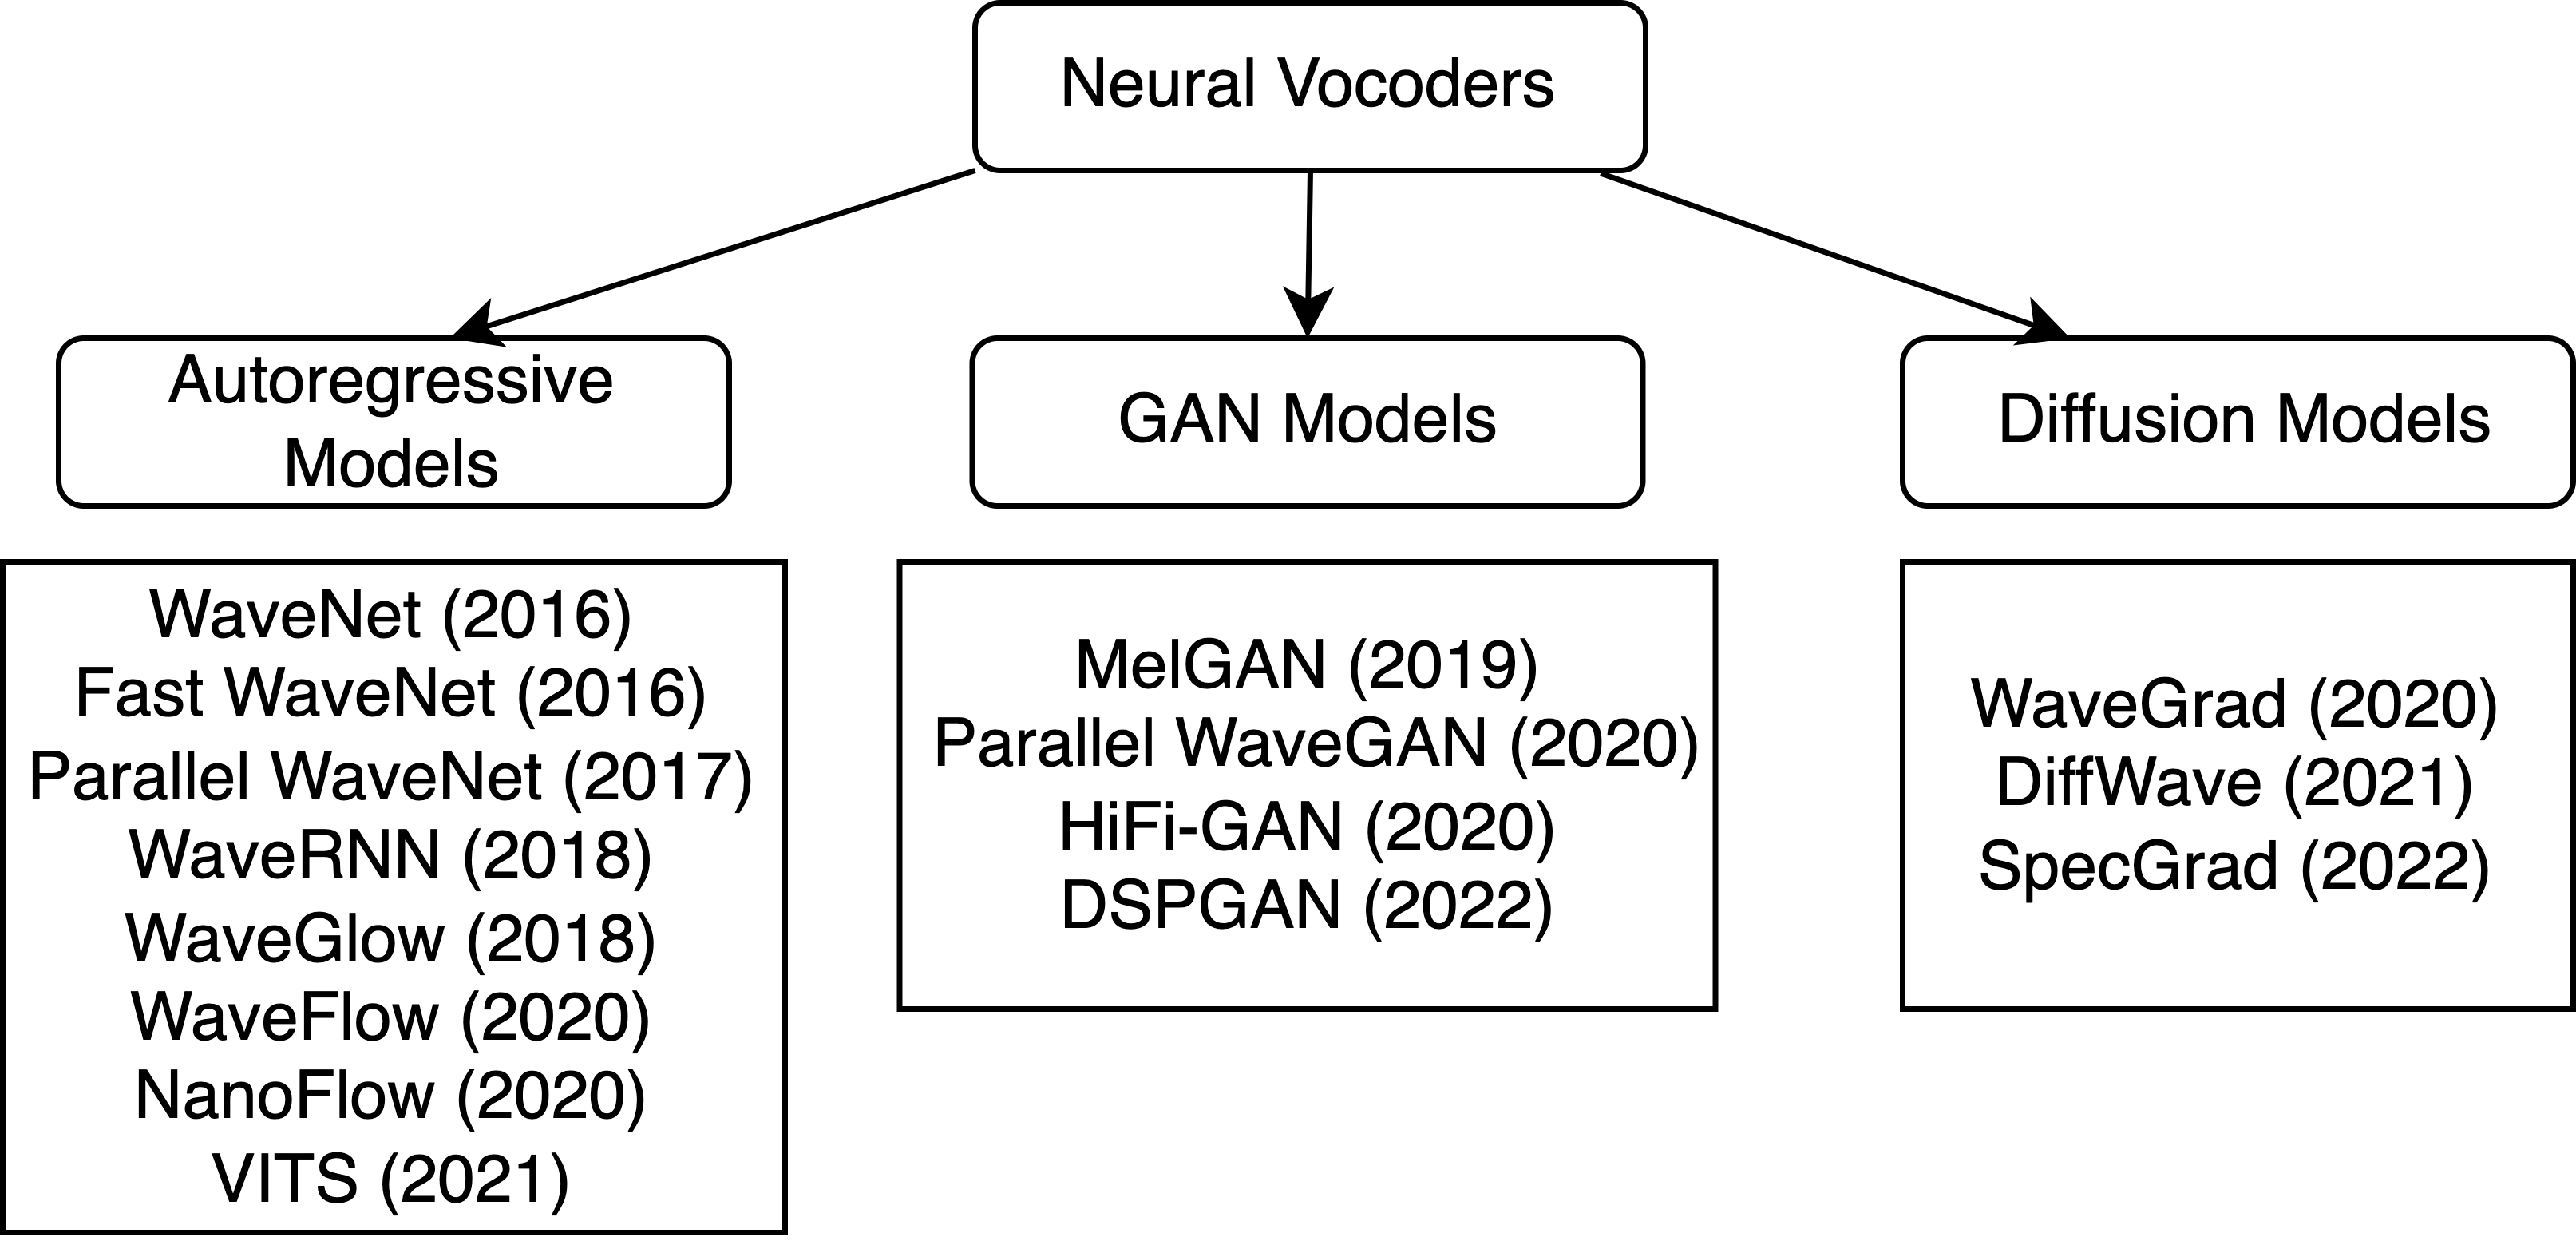
\includegraphics[width=0.99\linewidth]{figs/vocoders.png}
    \end{figure}
\end{frame}
%=======
\begin{frame}{Neural Vocoders}

\begin{table}[]
\begin{tabular}{|c|c|c|}
\hline
\textbf{\begin{tabular}[c]{@{}c@{}}Model \\ type\end{tabular}} & \textbf{Model}                                                   & \textbf{\begin{tabular}[c]{@{}c@{}}MOS on\\ LJ Speech\end{tabular}} \\ \hline
\multirow{2}{*}{\textbf{Autoregressive}}                       & WaveNet                                                          & 3.68                                                                \\ \cline{2-3} 
                                                               & WaveRNN                                                          & 3.96                                                                \\ \hline
\multirow{2}{*}{\textbf{GAN}}                                  & MelGAN                                                           & 3.73                                                                \\ \cline{2-3} 
                                                               & \begin{tabular}[c]{@{}c@{}}Parallel\\ WaveGAN\end{tabular}       & 3.99                                                                \\ \hline
\multirow{2}{*}{\textbf{Diffusion}}                            & WaveGrad                                                         & 3.85                                                                \\ \cline{2-3} 
                                                               & \textbf{DiffWave}                                                & \textbf{4.07}                                                       \\ \hline
\multirow{2}{*}{\textbf{}}                                     & Griffin-Lim                                                      & 3.68                                                                \\ \cline{2-3} 
                                                               & \textbf{\begin{tabular}[c]{@{}c@{}}Ground \\ Truth\end{tabular}} & \textbf{4.10}                                                       \\ \hline
\end{tabular}
\end{table}

    \myfootnotewithlink{https://arxiv.org/pdf/2112.03099.pdf}{AlBadawy et al., Vocbench: A Neural Vocoder Benchmark for Speech Synthesis, IEEE ICASSP, 2022}

\end{frame}
%=======
\section{WaveNet}
%=======
\begin{frame}{WaveNet}
    \begin{figure}
    	\centering
    	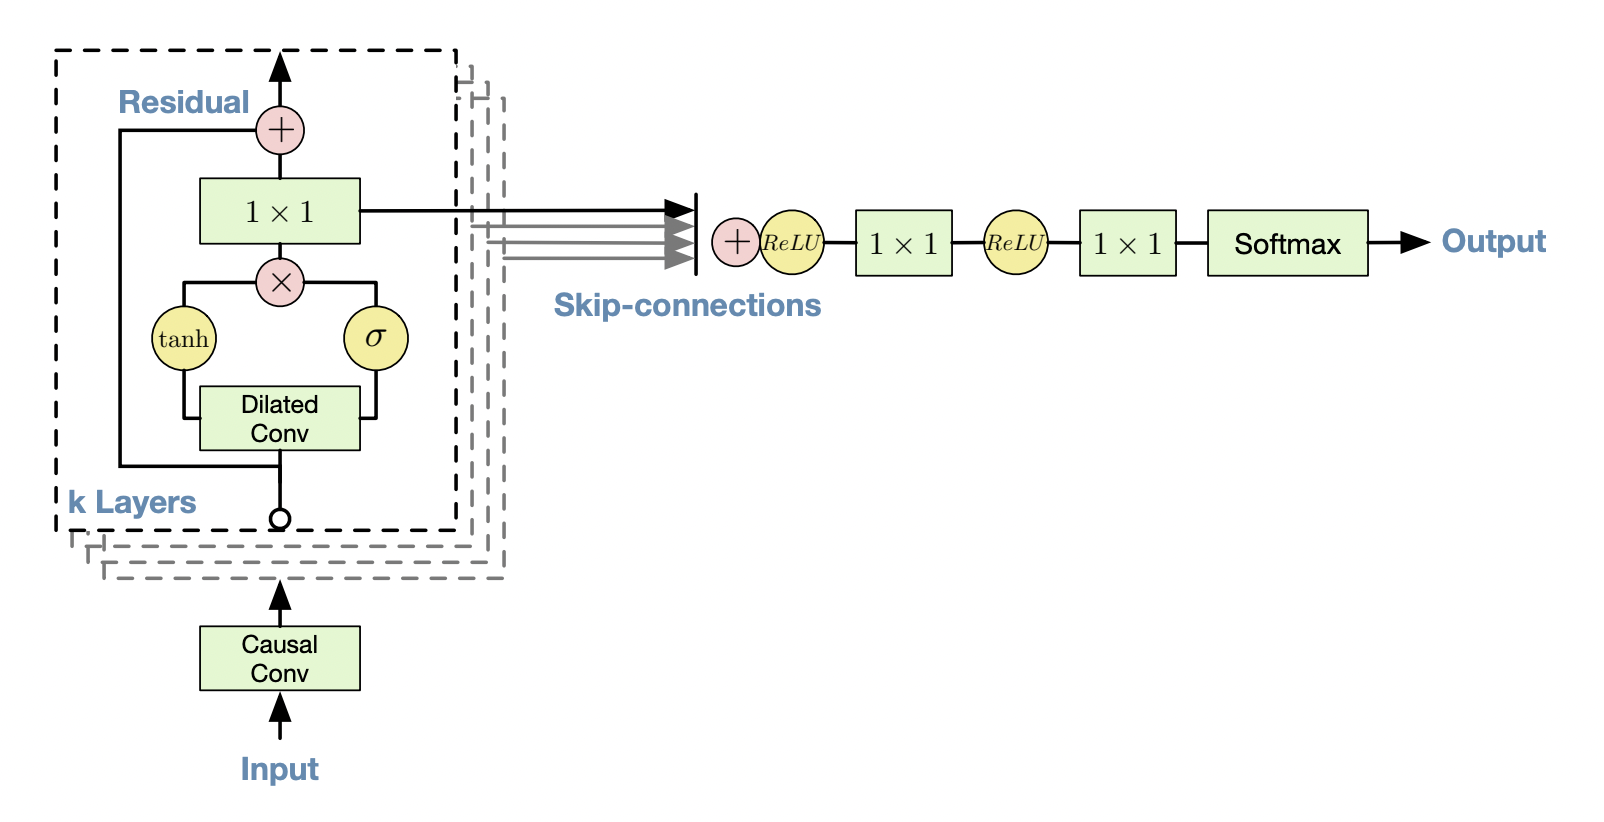
\includegraphics[width=0.8\linewidth]{figs/wavenet.png}
    	\caption{WaveNet architecture: uses \textbf{causal} dilated convolutions}
    \end{figure}
    \begin{itemize}
        \item The joint probability of a waveform $x = \{x_1, \cdots, x_T \}$:
        $p\left({\bf x}\right)=\prod_{t=1}^{T}p\left(x_{t}\mid x_{1:t-1}\right)$
        \item Each conditional $p\left(x_{t}\mid x_{1:t-1}\right)$ models the distribution for the timestamp $t$
    \end{itemize}
    
    \myfootnotewithlink{https://arxiv.org/pdf/1609.03499.pdf}{Oord et al., WaveNet: A Generative Model for Raw Audio, 2016}

\end{frame}
%=======
\begin{frame}{Causal Convolution}
    \begin{figure}
    	\centering
    	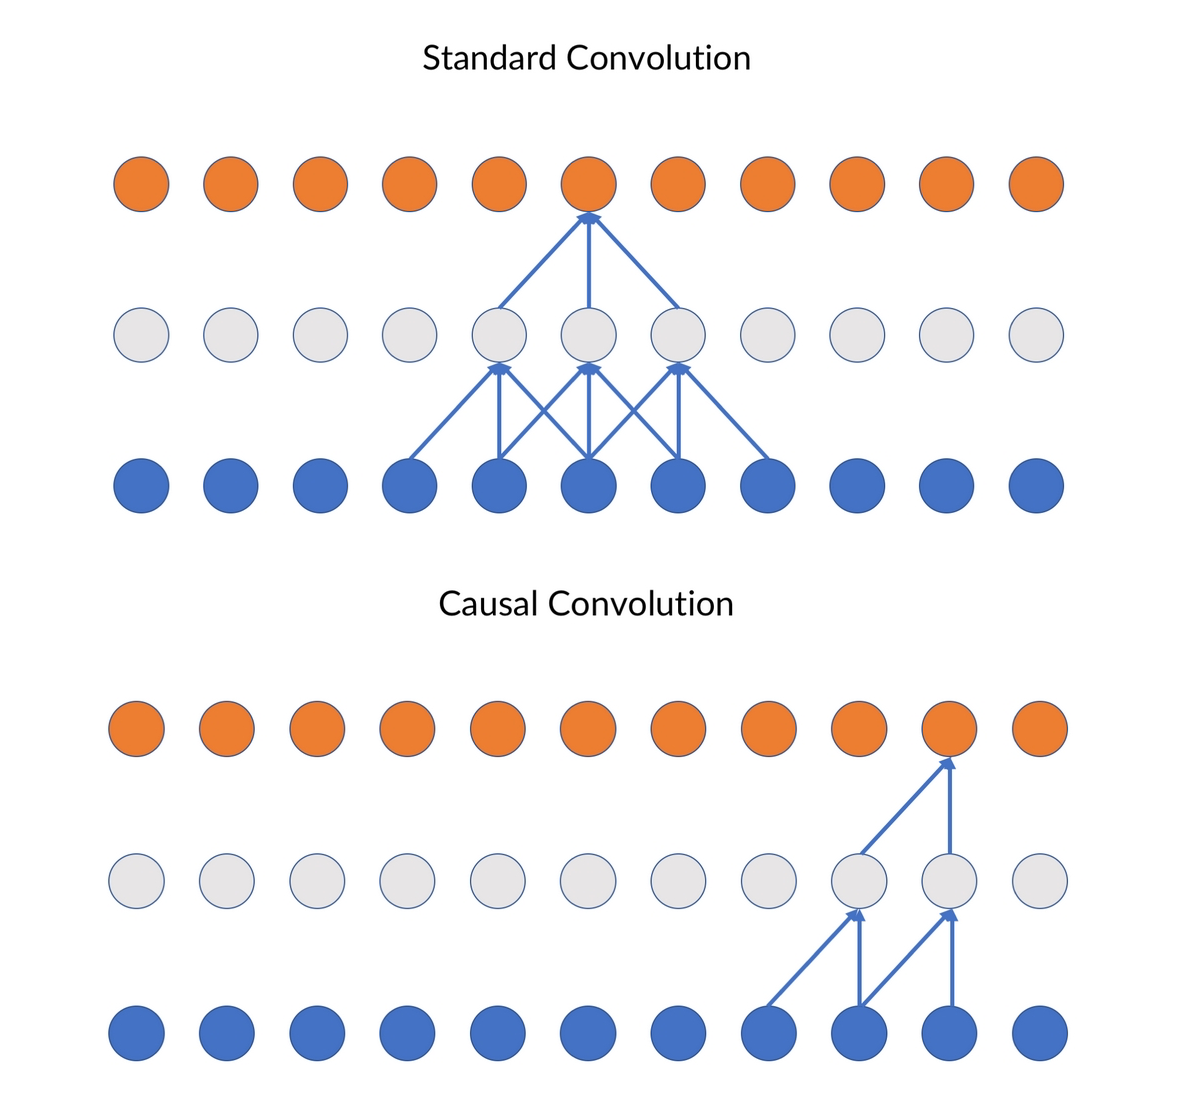
\includegraphics[width=0.7\linewidth]{figs/causal.png}
    	\caption{Standard vs causal convolutions. Causal makes convs autoregressive}
    \end{figure}
\end{frame}
%=======
\begin{frame}{Dilated Convolution}
    \begin{figure}
    	\centering
    	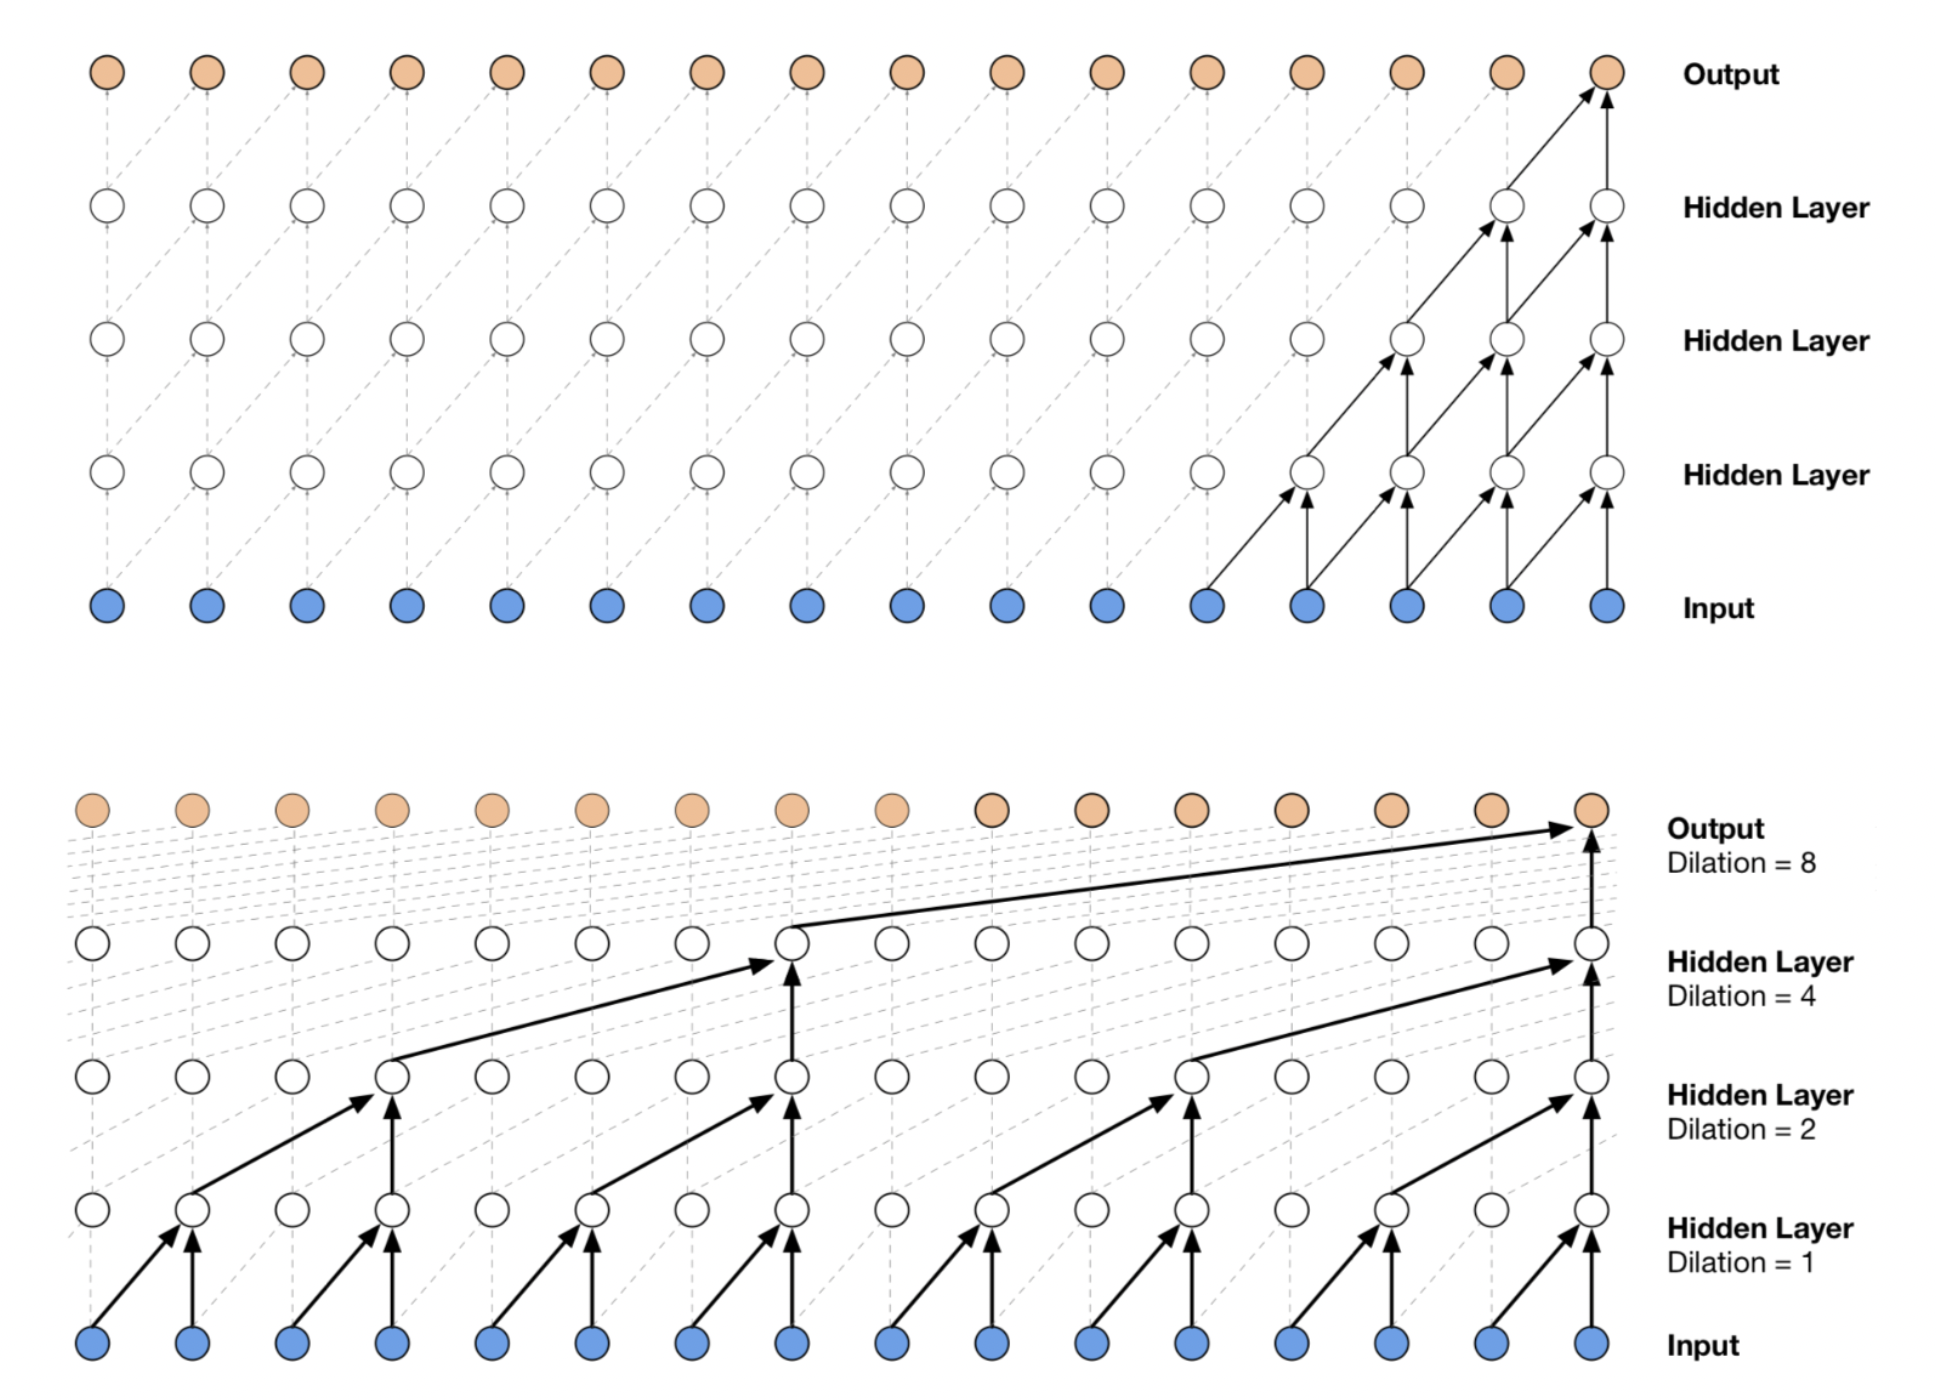
\includegraphics[width=0.9\linewidth]{figs/dilated_conv.png}
    	\caption{Non-dilated vs dilated causal convolutions. Dilated convs increase receptive fields}
    \end{figure}
\end{frame}
%=======
\begin{frame}{Conditional gated units}
    \begin{figure}
    	\centering
    	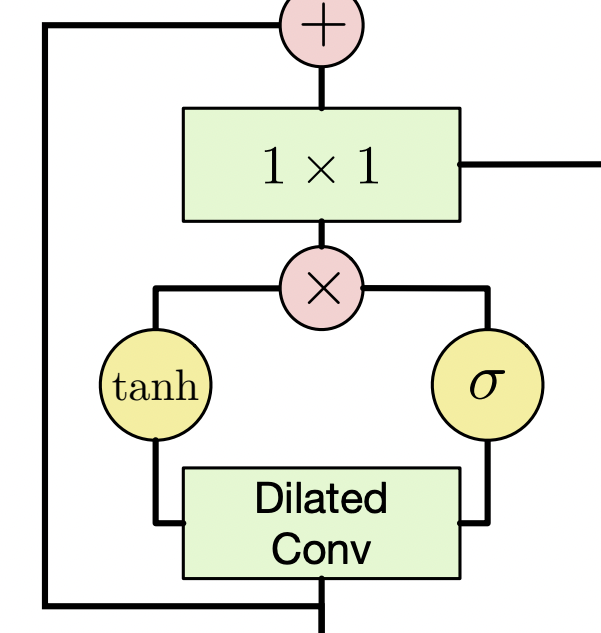
\includegraphics[width=0.35\linewidth]{figs/wavenet_gate.png}
    \end{figure}
    Gated activation unit as used in the gated PixelCNN + condition $\mathbf{y}$
    $$\mathbf{z}=\operatorname{tanh}\left(W_{f,k}*\mathbf{x}+V_{f,k}*\mathbf{y}\right)\odot\sigma\left(W_{g,k}*\mathbf{x}+V_{g,k}*\mathbf{y}\right).$$
    
    $*$ -- convolution, $\odot$ -- element-wise multiplication, $\sigma (\cdot)$ -- sigmoid function, $f$ and $g$ -- filter and gate, respectively, W -- learnable convolution filter, V -- learnable linear projection
\end{frame}
%=======
\begin{frame}{Mu Law Encoding}
    \begin{figure}
    	\centering
    	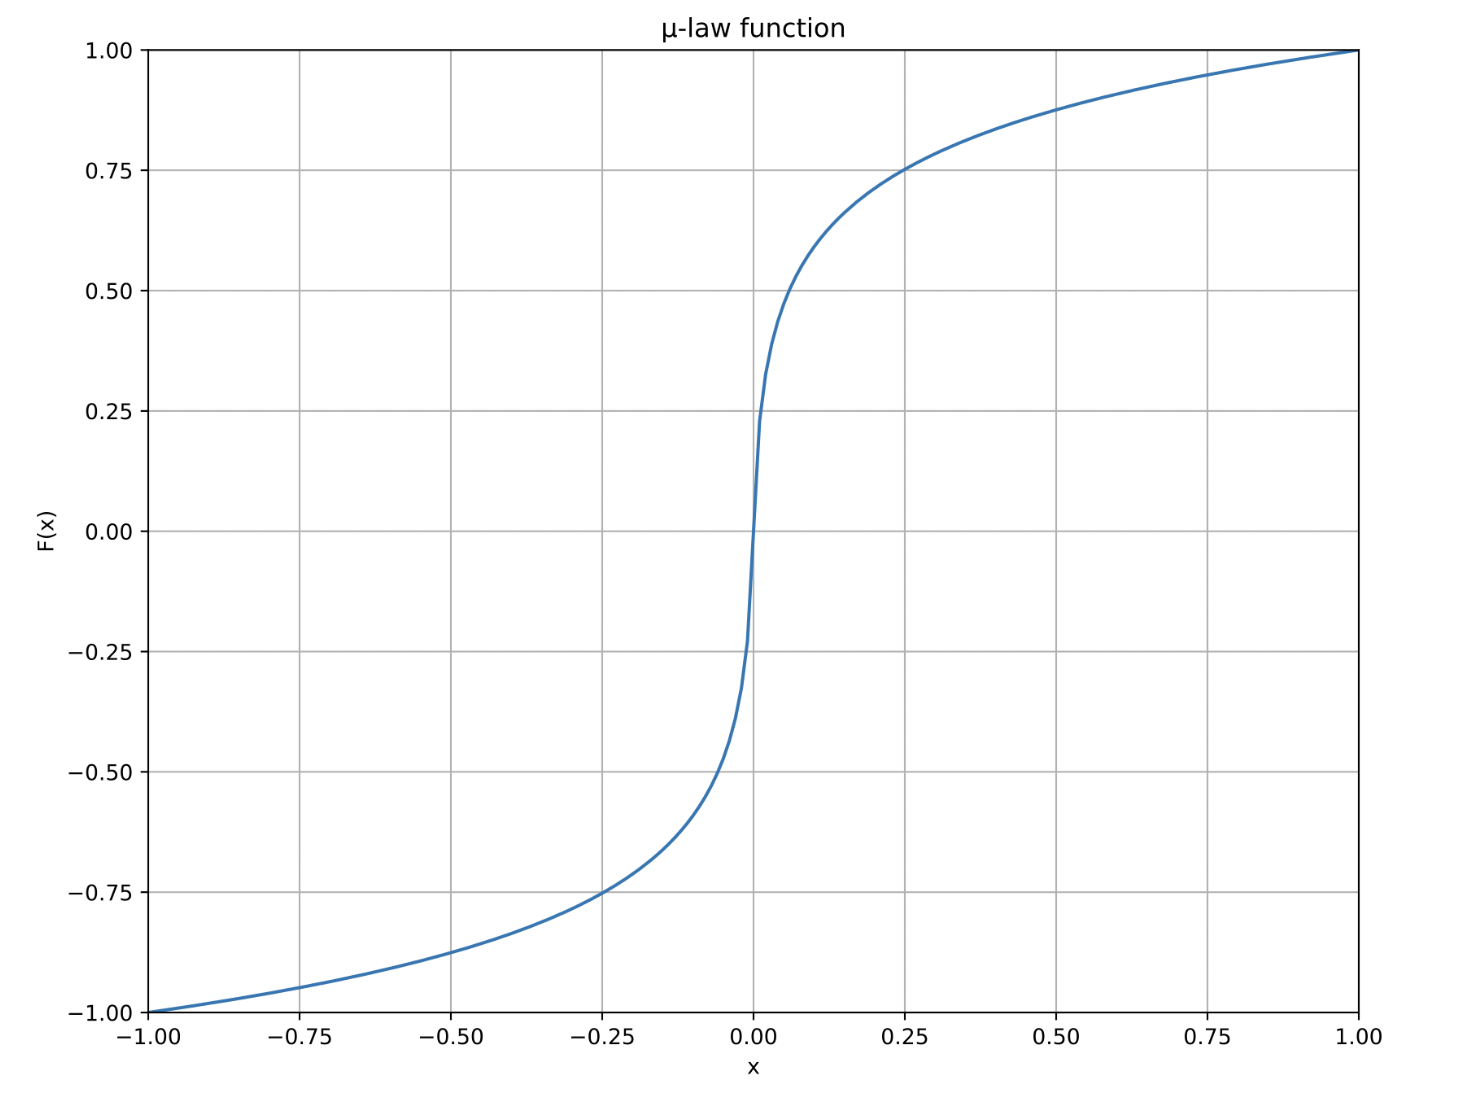
\includegraphics[width=0.5\linewidth]{figs/mu_law.png}
    \end{figure}
    \begin{itemize}
        \item Raw audio $\sim$ 16-bit integer values $\Rightarrow$ softmax layer need to output 65,536 probabilities per timestep
        \item Solution: apply a $\mu$-law transformation to the data, and then quantize it to 256 possible values:
        $$f\left(x_{t}\right)=\mathrm{sign}(x_{t})\frac{\ln\left(1+\mu\left|x_{t}\right|\right)}{\ln\left(1+\mu\right)}, ~~~ -1 < x_t < 1, \mu = 255$$
    \end{itemize}
\end{frame}
%=======
\section{Parallel WaveGAN}
%=======
\begin{frame}{Parallel WaveGAN}
    \begin{figure}
    	\centering
    	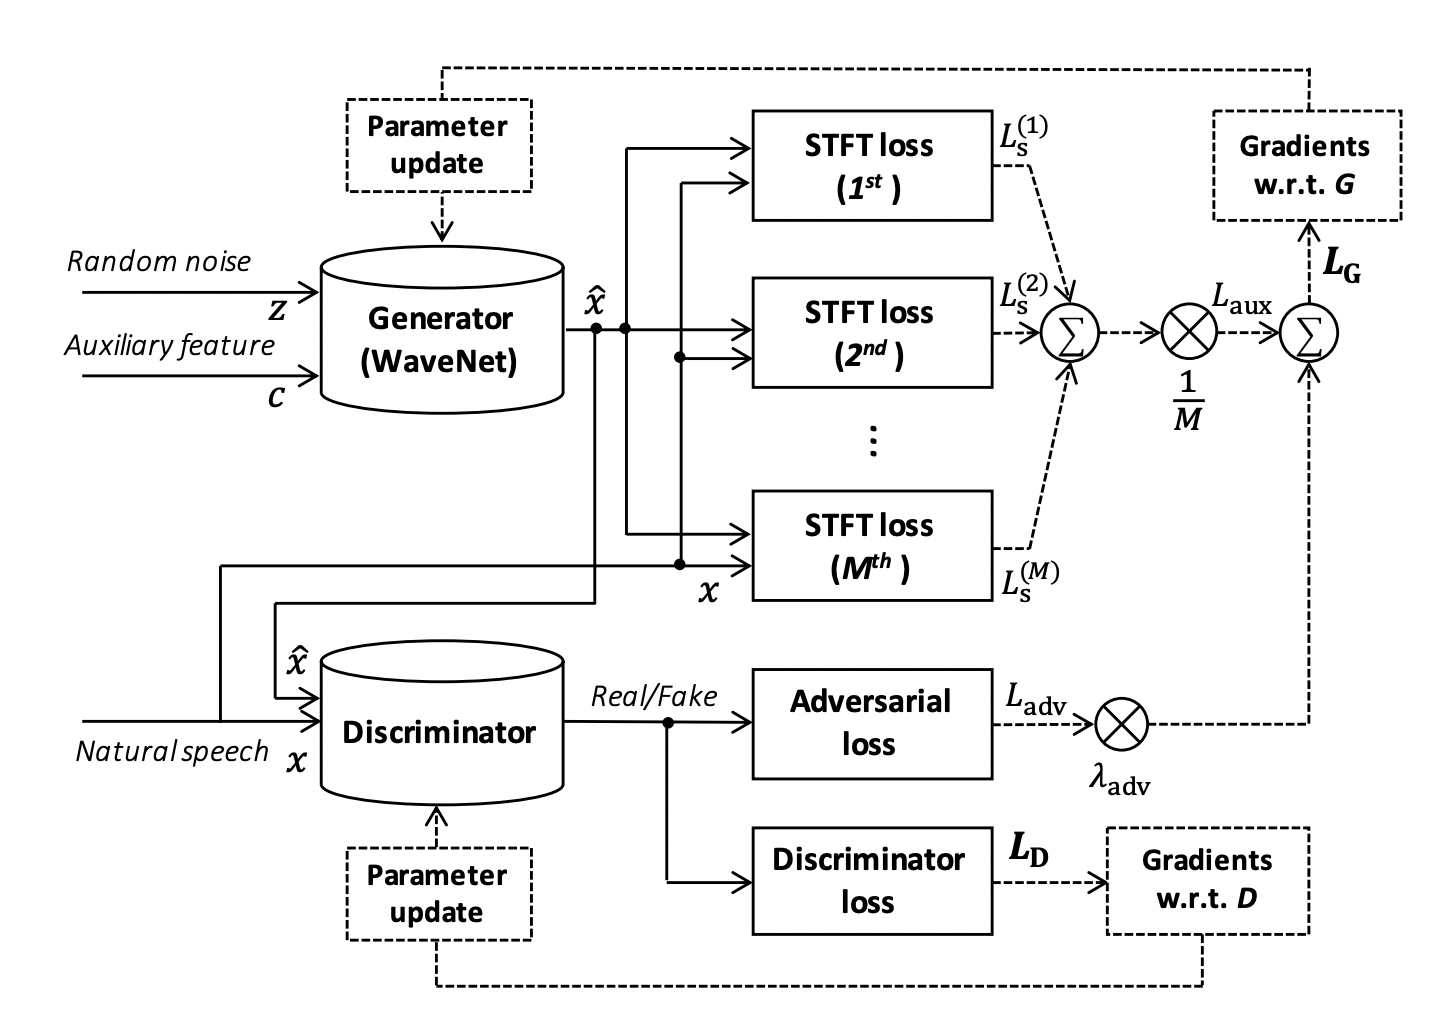
\includegraphics[width=0.7\linewidth]{figs/par_wavegan.png}
    	\caption{Parallel WaveGAN}
    \end{figure}

    \myfootnotewithlink{https://arxiv.org/pdf/1910.11480.pdf}{Yamamoto et al., Parallel Wavegan: A Fast Waveform Generation Model Based on Generative Adversarial Networks with Multi-Resolution Spectrogram, IEEE ICASSP, 2020}

\end{frame}
%=======
\begin{frame}{STFT Loss}
    \begin{figure}
    	\centering
    	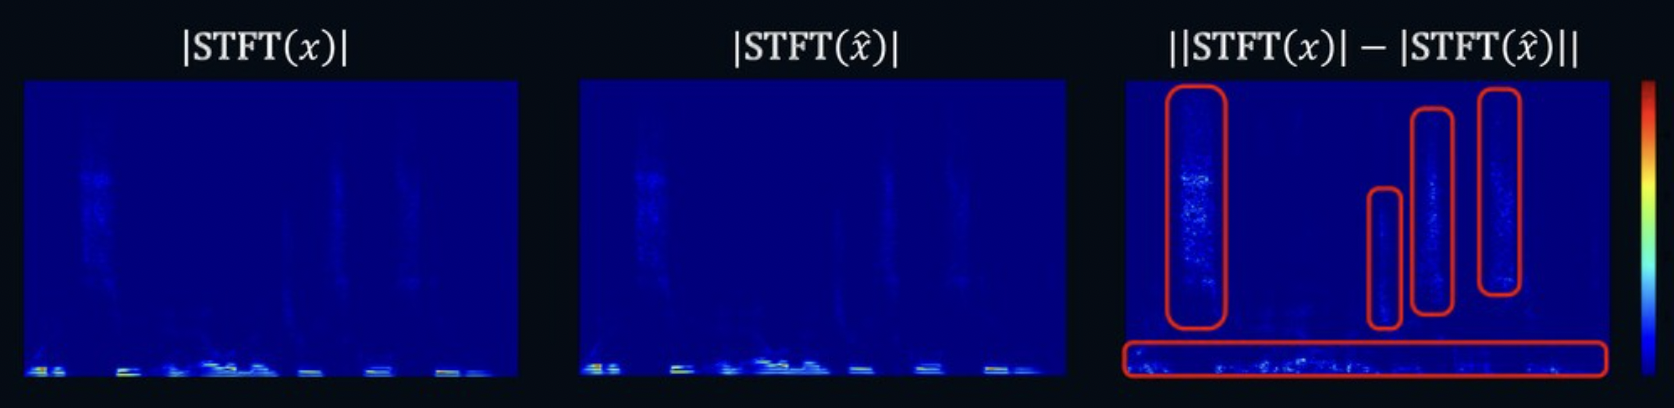
\includegraphics[width=0.7\linewidth]{figs/stft.png}
    \end{figure}
    
    $${\cal{L}}_{\mathrm{s}}(G)=\mathbb{E}_{\mathbf{z}\sim p(\mathbf{z}),\mathbf{x}\sim p_{data}}\left[\cal L_{\mathrm{sc}}(\mathbf{x},{\mathbf{\hat{x}}})+\cal{L}_{\mathrm{mag}}(\mathbf{x},{\mathbf{\hat{x}}})\right]$$
    
    $${\cal{L}}_{\mathrm{sc}}(\mathbf{x},\mathbf{\hat{x}})=\frac{\left\Vert \left|\mathrm{STFT}(\mathbf{x})\right|-\left|\mathrm{STFT}^{\mathrm{T}}(\mathbf{\hat{x}})\right|\right\Vert}{\left\Vert \left|{STFT}(\mathbf{x})\right|\right\Vert_F}$$
    
    $${\cal L}_{\mathrm{mag}}(\mathbf{x},\mathbf{\hat{x}})={\frac{1}{N}}\left\Vert\log\left|\mathrm{STFT}(\mathbf{x})\right|-\log\!\left|\mathrm{STFT}(\mathbf{\hat{x}})\right| \right\Vert_1$$
    
    $${\cal L}_{\mathrm{aux}}(G)={\frac{1}{M}}\sum_{m=1}^{M}{\cal L}_{\mathrm{s}}^{(m)}(G), \text{M -- number of STFT losses}$$
    
    \myfootnotewithlink{https://arxiv.org/pdf/1810.11945.pdf}{Takaki et al., STFT Spectral Loss for Training a Neural Speech Waveform Model, IEEE ICASSP, 2019}

\end{frame}
%=======
\begin{frame}{GAN Loss}
    
    \begin{itemize}
        \item Discriminator Loss:
        $${\cal L}_{\mathrm{D}}(G,D)=\mathbb{E}_{\mathbf{x}\sim p_{\mathrm{data}}}[(1-D(\mathbf{x}))^{2}]+\mathbb{E}_{\mathbf{z}\sim N(0,I)}[D(G(\mathbf{z}))^{2}]$$
        
        \item Generator Loss
        $$L_{\mathrm{adv}}(G,D)=\mathbb{E}_{\mathbf{z}\sim N(0,I)}\left[(1-D(G(\mathbf{z})))^{2}\right]$$
        
        $$L_{\mathrm{G}}(G,D)=L_{\mathrm{aux}}(G)+\lambda_{\mathrm{adv}}L_{\mathrm{adv}}(G,D)$$
    \end{itemize}


\end{frame}
%=======
\section{DiffWave}
%=======
\begin{frame}{Diffusion models idea}
        \begin{figure}
    	\centering
    	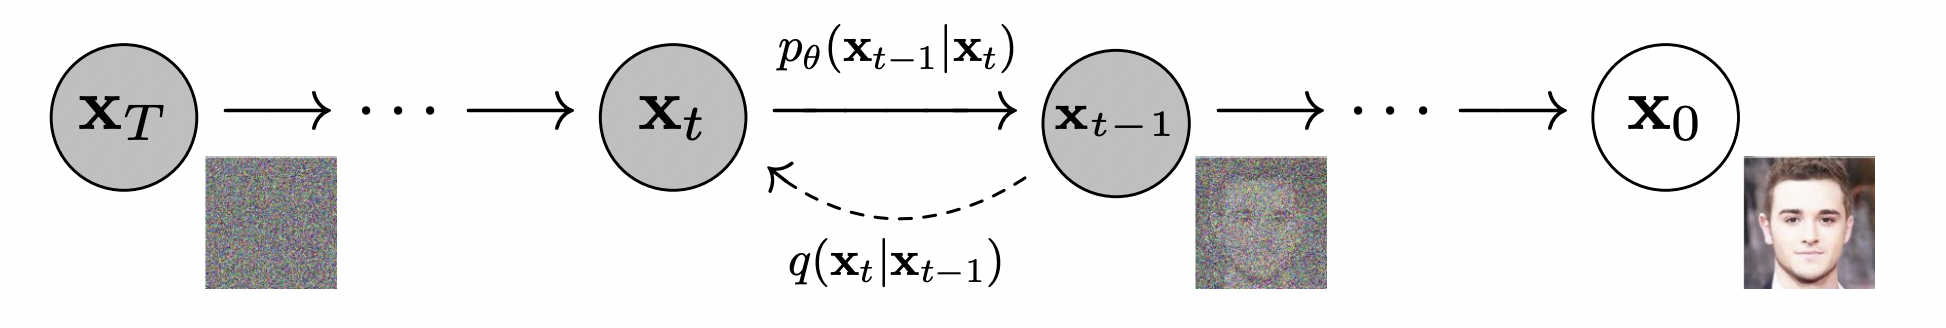
\includegraphics[width=0.99\linewidth]{figs/diffusion.png}
    \end{figure}
    \begin{itemize}
        \item \textbf{Diffusion probabilistic model}: parameterized Markov chain from data $x_0$ to the latent variable $x_T$
        $$q(x_{1},\cdot\cdot\cdot\cdot\cdot x_{T}|x_{0})=\prod_{t=1}^{T}q(x_{t}|x_{t-1})$$
        
        \item \textbf{Reverse process}: Markov chain from $x_T$ to $x_0$ parameterized by $\theta$:
        $$p_{\mathrm{latent}}(x_{T})=\mathcal{N}(0,I),\ ~~~p_{\theta}(x_{0},\cdot\cdot\cdot,x_{T-1}|x_{T})=\prod_{t=1}^{T}p_{\theta}(x_{t-1}|x_{t})$$
        
    \end{itemize}
    
    \myfootnotewithlink{https://arxiv.org/pdf/2006.11239.pdf}{Ho et al., Denoising Diffusion Probabilistic Models, NeurIPS Proceedings, 2020}

\end{frame}
%=======
\begin{frame}{DiffWave}
        \begin{figure}
    	\centering
    	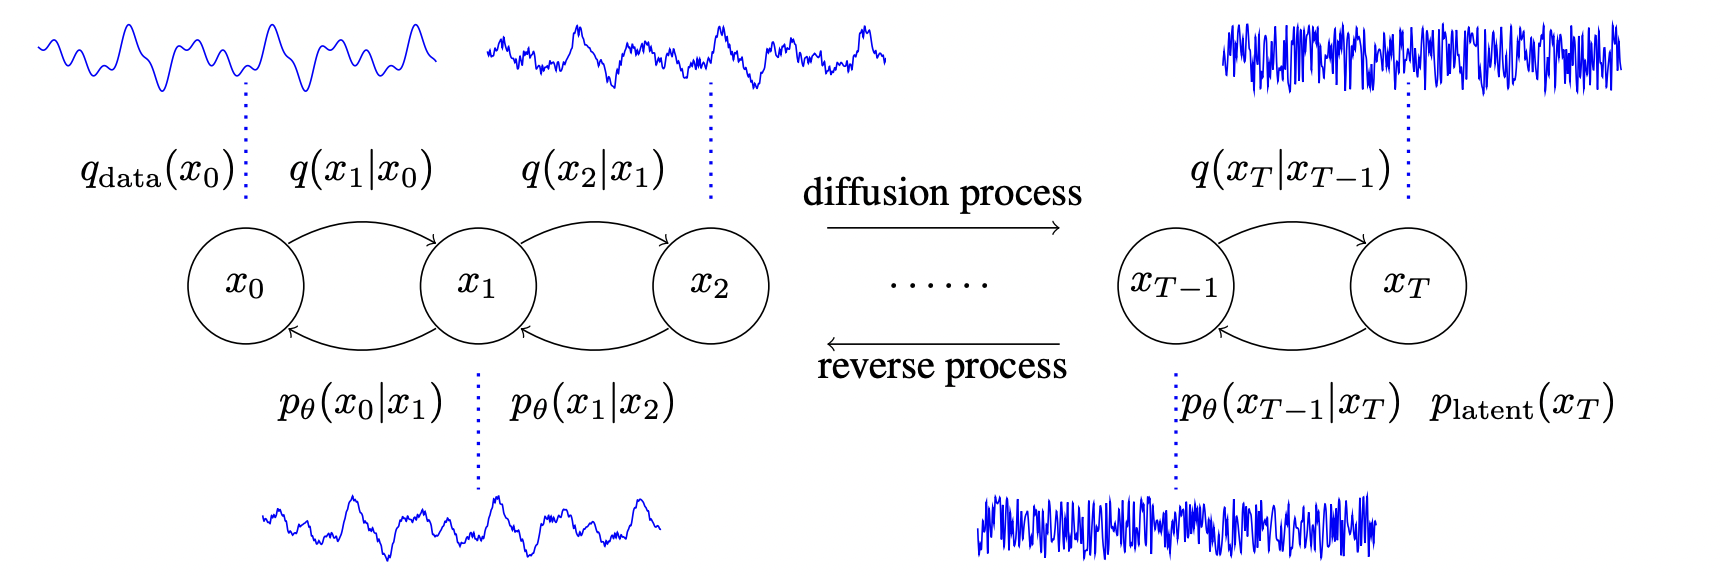
\includegraphics[width=0.8\linewidth]{figs/diffusion_audio.png}
    \end{figure}
    
    \begin{itemize}
        \item \textbf{Sampling}: reverse process $x_{T} \sim \mathcal{N}(0, I)$, $x_{t-1} \sim p_{\theta}(x_{t-1}|x_t)$ for $t = T, T - 1, \cdots , 1$. $x_0$ -- sampled data.
        \item \textbf{Training}: $p_{\theta}(x_{0})=\int p_{\theta}(x_0, \cdots, x_{T-1}|x_{T})\cdot p_{\mathrm{latent}}(x_{T}) \mathbf{d}x_{1;T}$ (likelihood) is intractable to calculate $\Rightarrow$ model trained by maximizing its variational lower bound (ELBO):
        \begin{multline*}
        \mathbb{E}_{q_{\mathrm{data}}(x_{0})}\log p_{\theta}(x_{0}) \geq \\
        \geq \mathbb{E}_{q(x_{0},\cdots,x_T)}\log{\frac{p_{\theta}(x_{0},\cdots,x_{T-1}|x_{T})\cdot p_{\mathrm{latent}}(x_{T})}{q(x_{1},\cdots,x_{T}|x_{0})}}:={\mathrm{ELBO}}
        \end{multline*}
    \end{itemize}
    
    \myfootnotewithlink{https://arxiv.org/pdf/2009.09761.pdf}{Kong et al., DiffWave: A Versatile Diffusion Model for Audio Synthesis, ICLR, 2021}

\end{frame}
%=======
\begin{frame}{DiffWave: advantages}
    \begin{itemize}
        \item \textbf{Non-autoregressive}: much faster than WaveNet
        \item \textbf{Compact model}: smaller footprint than flow-based models
        \item No auxiliary losses in training (e.g., spectrogram-based losses): \textbf{no mode collapse} like in GANs/VAEs
    \end{itemize}

\end{frame}
%=======
\end{document} 
